%-------------------------------------------------------------------------------
\section{Evaluation}
%-------------------------------------------------------------------------------
Sanity check: \newline
%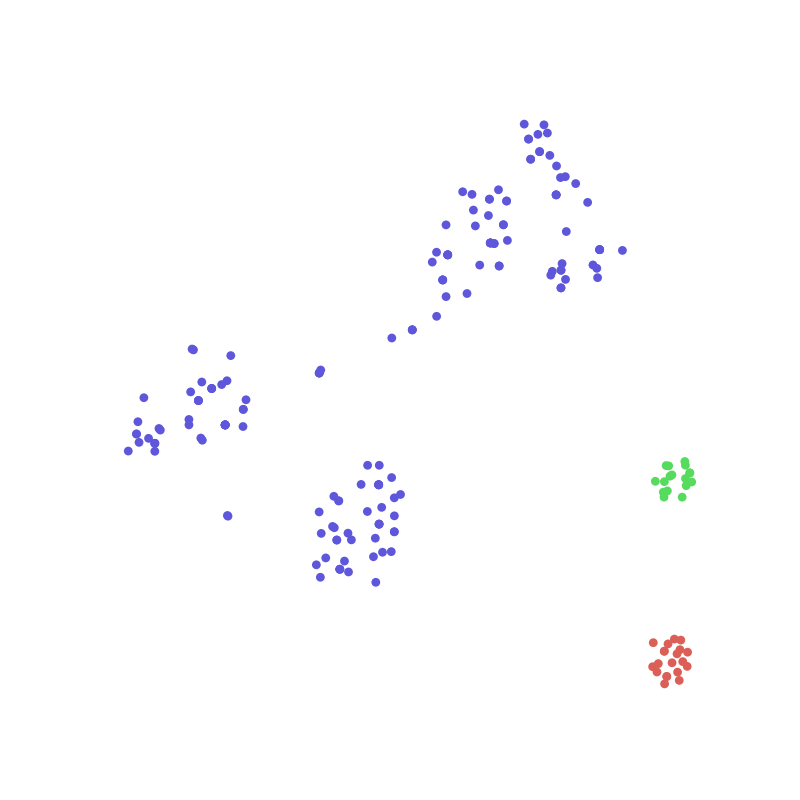
\includegraphics[scale=0.2]{tsne_viz.png}
\begin{itemize}
\item Classification: \newline 
Why classification? 
We are able to learn clusters accurately, but the problem is that using the clusters for predictive analysis performs poorly. The reason is that clusters are diffuse and in order to predict if a graph is in a cluster or not, the arithmetic mean of all pints in the cluster is computed. Doing so, however, results in information loss and leads to inaccurate results.

I started with a set of good graphs and a restricted set of test graphs
Classification worked perfectly when we have 16-dimensional vectors for the nodes \ newline
%\includegraphics[scale=0.4]{logistic_2d.png} \newline
%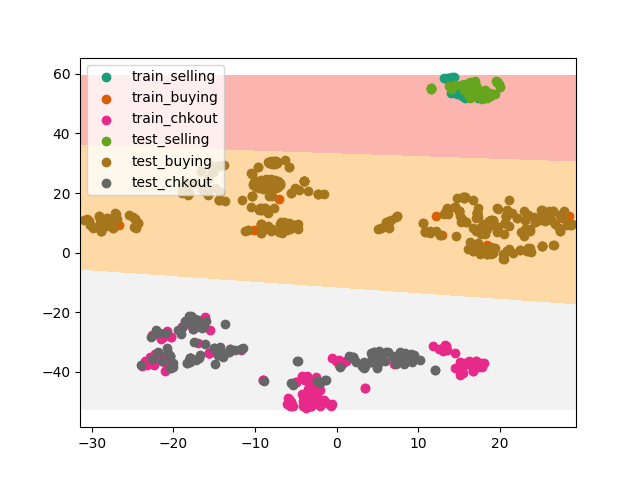
\includegraphics[scale=0.4]{test_logistic_2d.png} \newline

Q: Can we reduce the dimensions further?
When the dimensions were reduced to 4, a few graphs were mis-classified but not many  i.e. earlier there were no misclassification, now 1 in 575 graphs was misclassified

Take-away: Only small amount of information was required for classification, enabling compression

\item Predicting missing nodes and edges:  \newline
The way the problem is set up is that we have a graph that may be missing some nodes and/or edges. We have a set of complete graphs. Which one of them is the completion to our graph?
We can use euclidean distance between the representation for our graph and the target graph and choose the one that minimizes it. The traditional way to do this , however, is to use graph edit distance. 

Q: Do our results approximate computing the graph edit distance approach? 
To compute this, we implemented both approaches and then computed mean, median and mode for each of the two approaches. As the number of dimensions increased from 4 to 16, the gap between the two approaches narrowed. 

Q: Can we eliminate this gap? What if we choose number of dimensions to be 128?
Turns out 128 dimensions is only a slight improvement over 16

Take away: This question requires more information to be retained as compared with classification.
\end{itemize}

